\documentclass{ctexbeamer}
\usetheme{Hannover}
\usecolortheme{rose}
\linespread{1.1}
\usepackage{listings}
\lstset{language=Python,frame=single,basicstyle=\scriptsize\ttfamily,keywordstyle=\color{blue!70}\bfseries,showstringspaces=false,commentstyle=\ttfamily\color{green!40!black},breaklines=true}

\def\mathfamilydefault{\rmdefault}

\title{Python爬虫踩坑记录}
\date{\today}
\author[胡沐彦]{计97 胡沐彦}

\begin{document}

\begin{frame}
	\titlepage
\end{frame}

\section{爬取思路}
\begin{frame}{爬取思路}
	\begin{itemize}
		\item 运行环境:Ubuntu 20.04,爬取豆瓣电影信息与演员信息
		\pause \item 电影与演员的爬取分开进行
		\pause \item 用\texttt{urllib}库进行网页页面的获取,然后利用正则表达式库\texttt{re}提取页面上的信息,最后用\texttt{json}库将信息以json格式保存
	\end{itemize}
\end{frame}

\section{网页页面获取}
\begin{frame}{网页页面获取}
	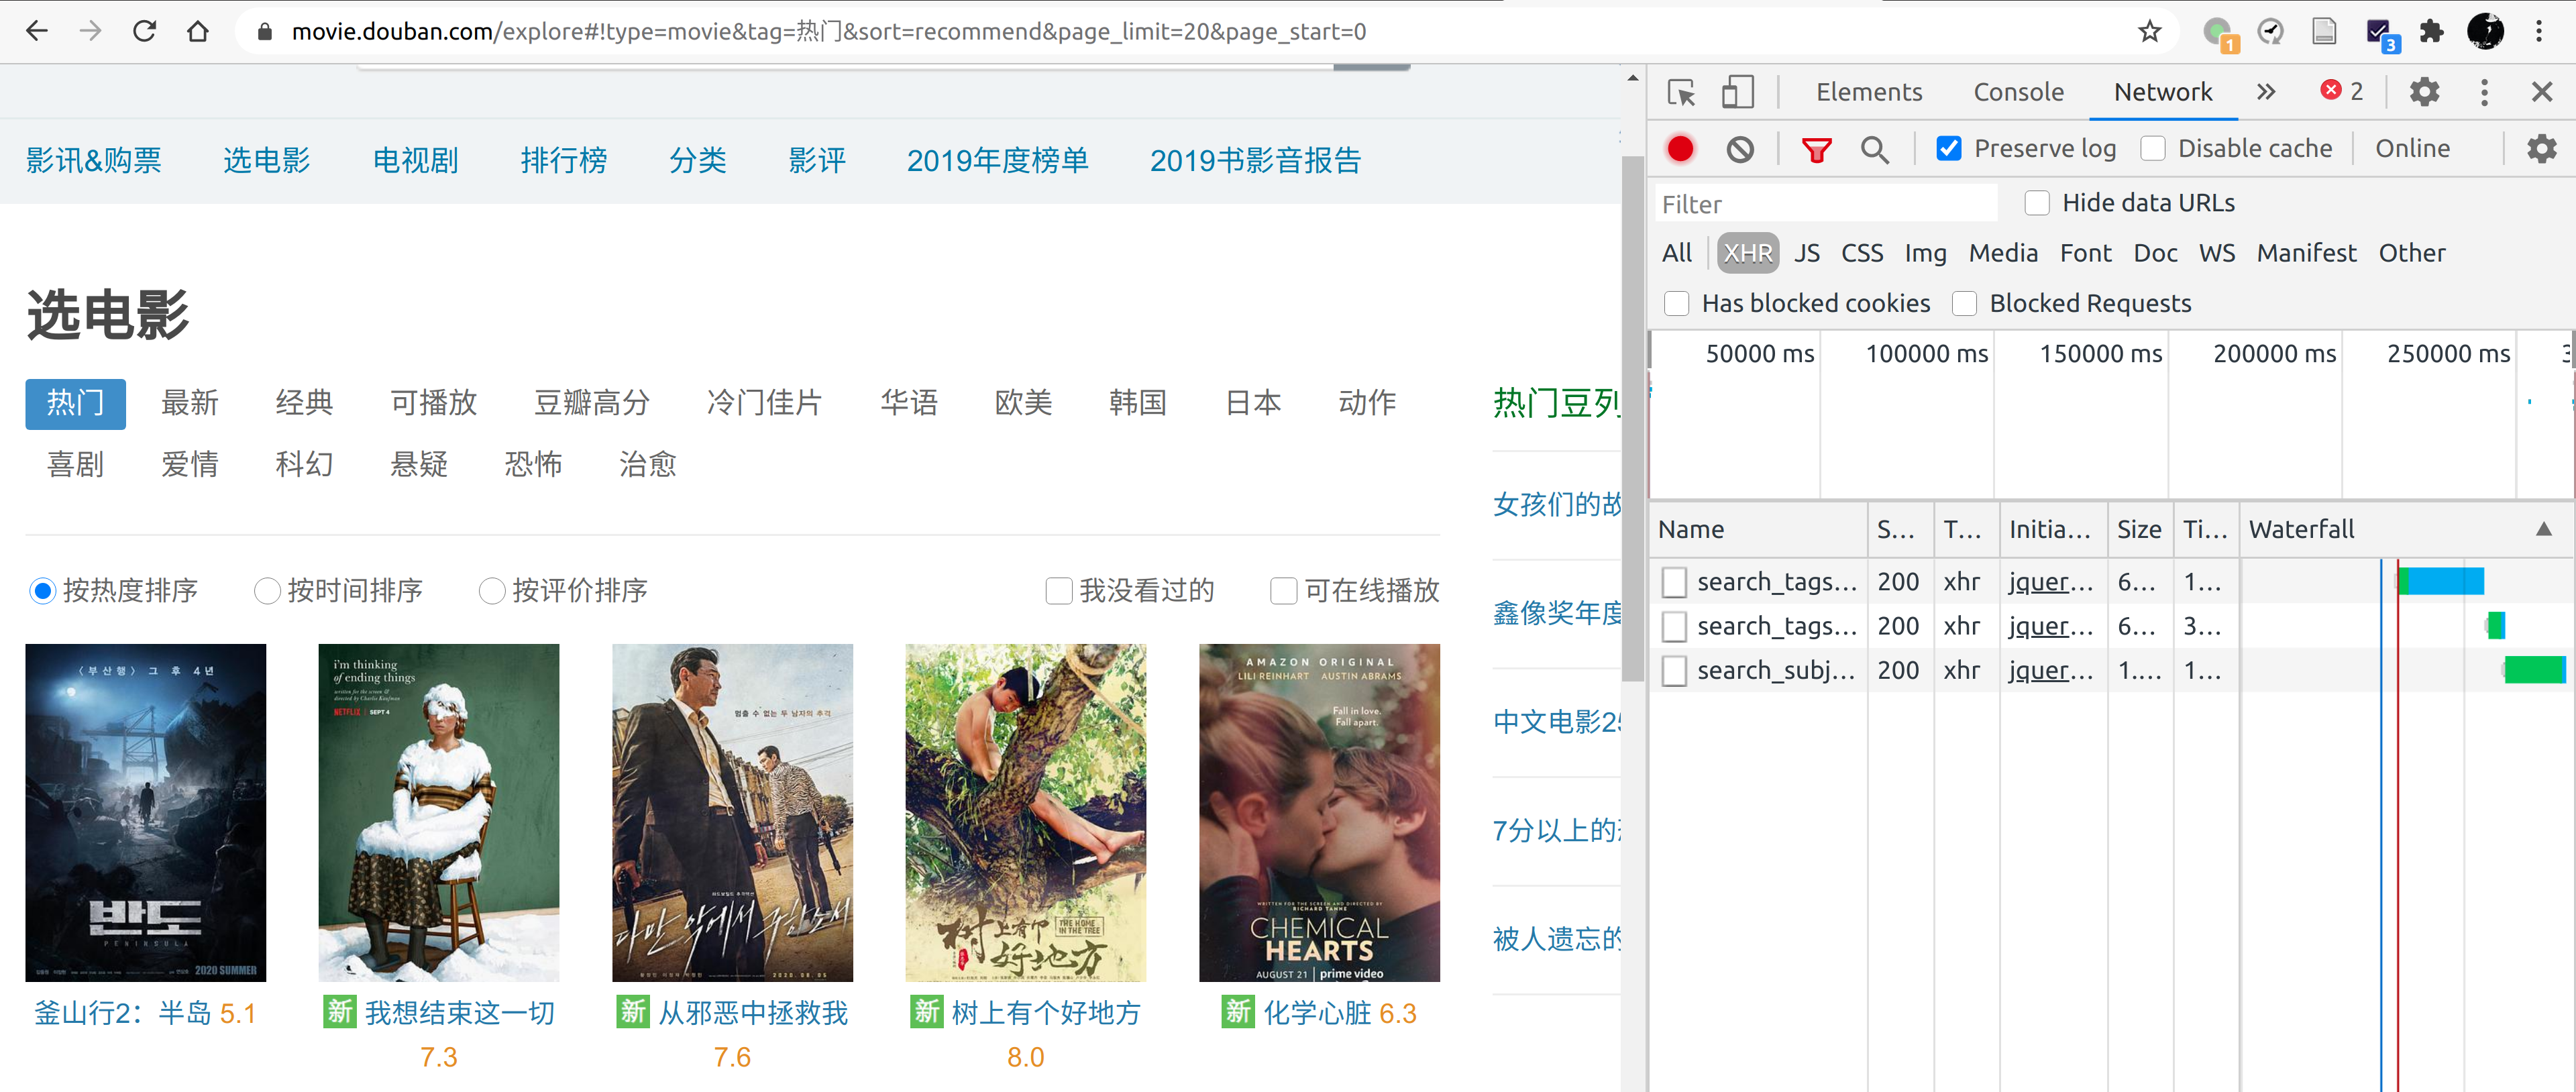
\includegraphics[width=\textwidth]{f12.png}
	无法直接从该页面源码中获取电影链接,用chrome浏览器自带的devtools中记录network activity功能抓取到需要的链接
\end{frame}
\begin{frame}{网页页面获取}
	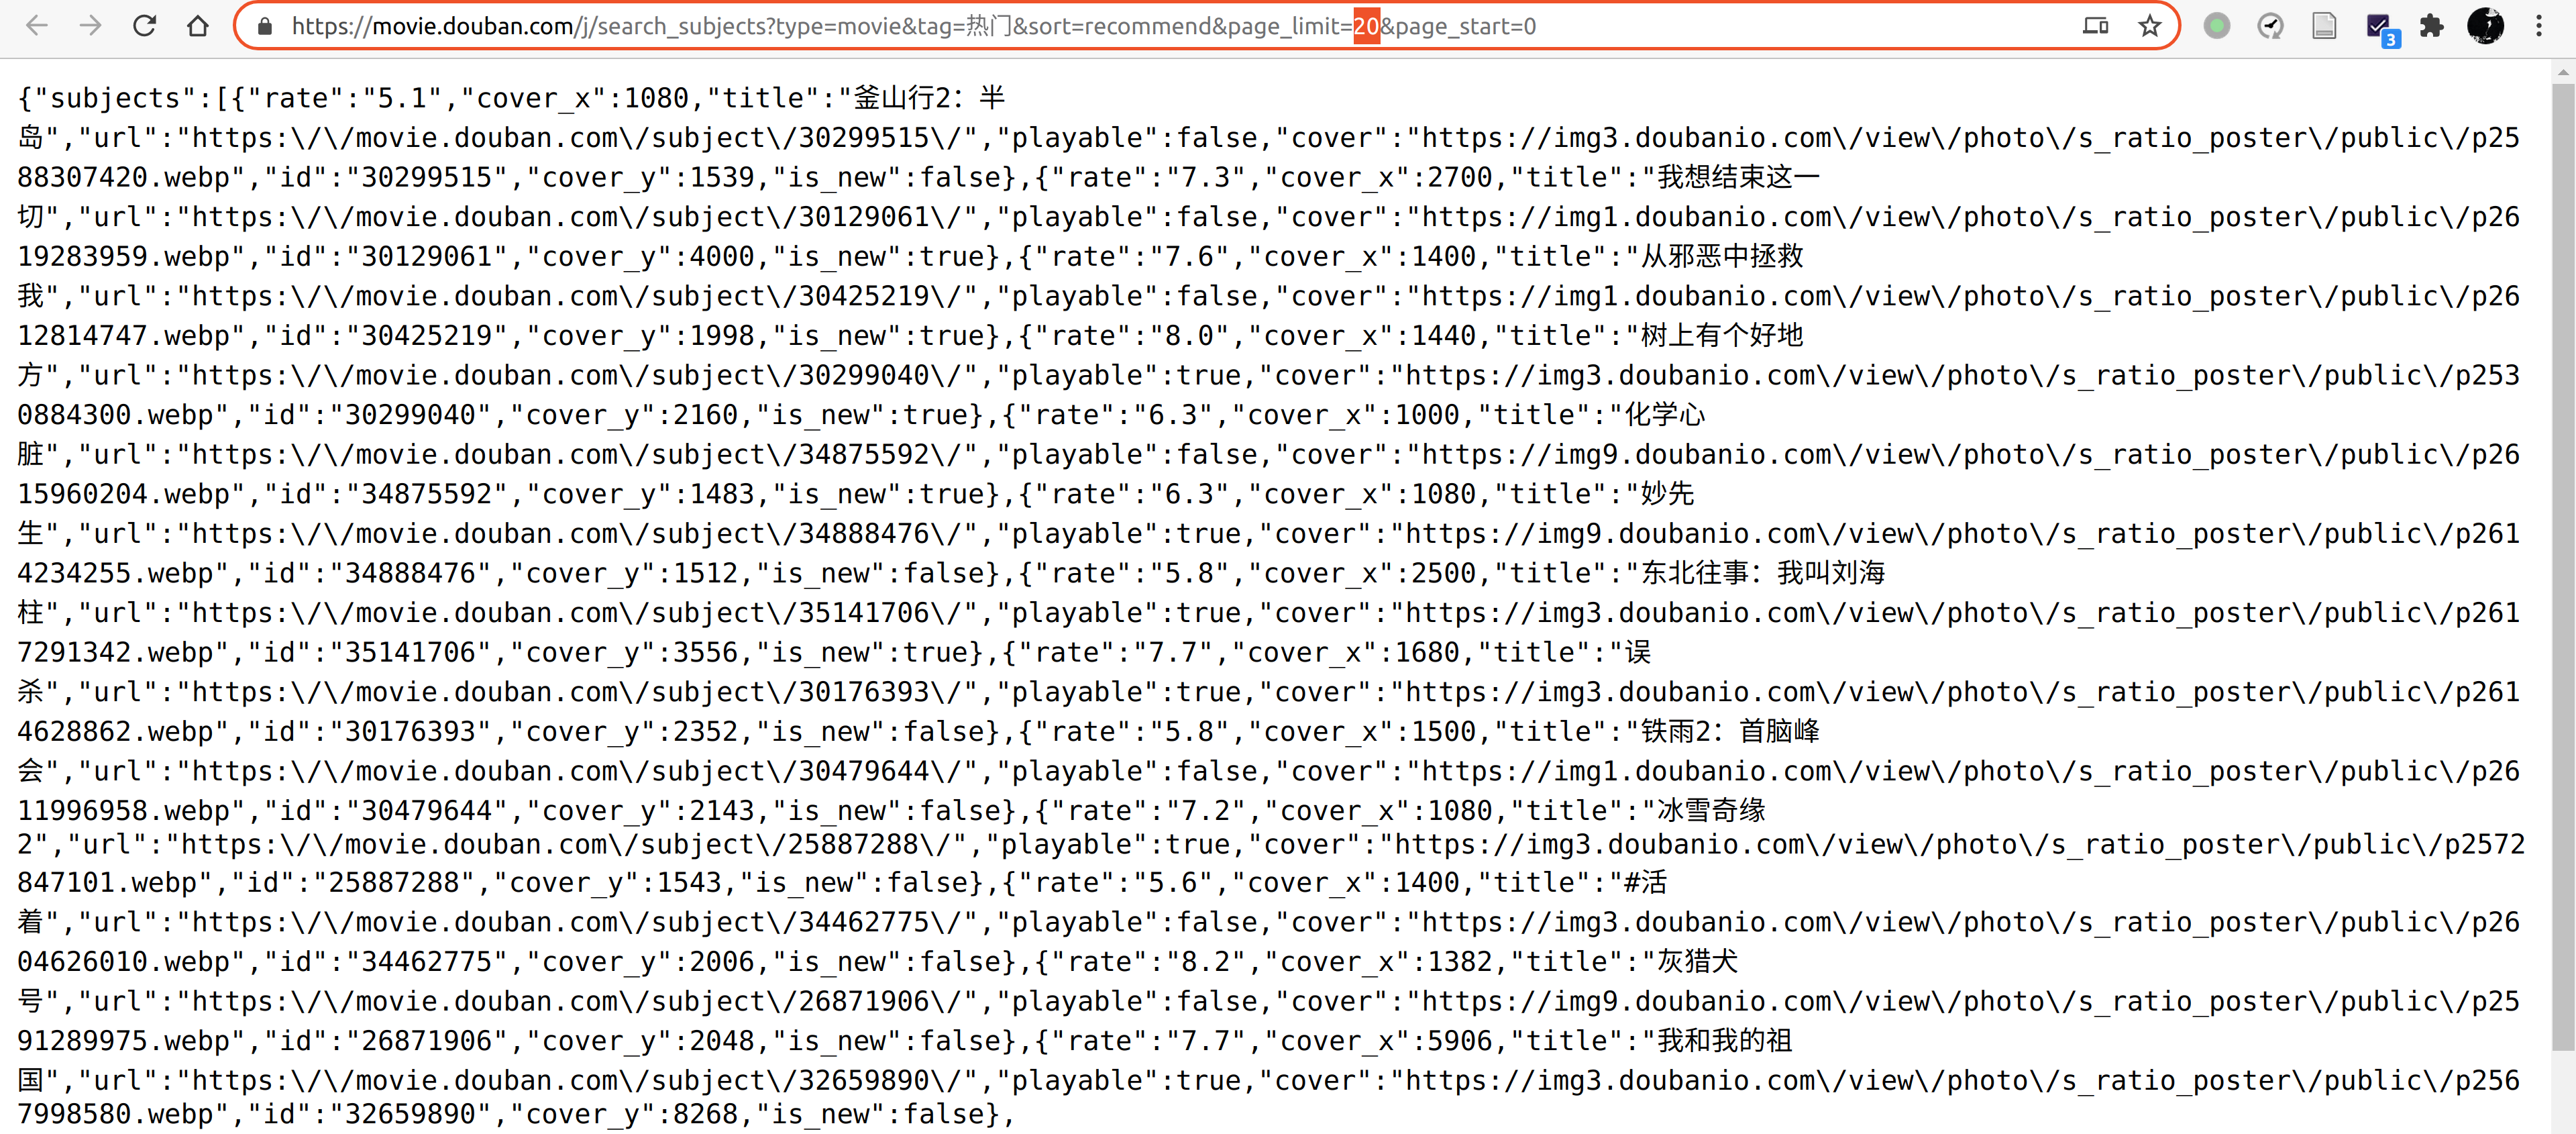
\includegraphics[width=\textwidth]{background.png}
	通过观察,调整链接中的\texttt{page\_limit}获取所有电影列表
\end{frame}
\begin{frame}[fragile]
	\frametitle{网页页面获取}
\begin{lstlisting}
req = Request(url)
req.add_header("User-Agent", Header)
sourceCode = urlopen(req).read().decode("utf-8")
\end{lstlisting}
	\begin{itemize}
		\item \texttt{Header}为一个消息头字符串:\texttt{Mozilla/5.0 (Windows NT 6.1; Win64; x64) AppleWebKit/537.36 (KHTML, like Gecko) Chrome/76.0.3809.100 Safari/537.36}
		\pause \item 加入后可降低被反爬虫的概率
		\begin{itemize}
			\item 实测在随机\texttt{sleep} $2\sim 3$s的爬取速度下不会被封
		\end{itemize}
	\end{itemize}
\end{frame}

\section{页面信息提取}
\begin{frame}{基本信息提取}
	根据观察HTML代码设计尽可能准确的正则表达式
	
\includegraphics[width=\textwidth]{duration.png}
	\vspace{-4ex}
	\begin{itemize}
		\item 如电影长度为\texttt{int(re.search(r'<span property="v:runtime" content="([0-9]+)">', html).group(1))}
	\end{itemize}
	用\texttt{os.system}运行\texttt{wget}命令下载图片,以电影/演员的豆瓣ID作为保存文件名
\end{frame}
\begin{frame}{豆瓣网页的一些小trick}
	\begin{itemize}
		\item 豆瓣电影有专门的影评网页(电影链接后加\texttt{/reviews}),爬取影评更方便
		\pause \item 有些内容可能需要点击“显示全部”查看完整内容,在HTML源码中一般显示在\texttt{<span class="all hidden">}之后
	\end{itemize}
\end{frame}
\begin{frame}{Python的一些小trick}
	\begin{itemize}
		\item 网页源代码中含有HTML转义字符,可以用\texttt{html.unescape}转换
		\pause \item 获得满足正则表达式\texttt{pattern}的前$k$个匹配可以用\texttt{for x in isslice(re.finditer(pattern, string), k)}
		\pause \item 输出为json文件用\texttt{json.dumps},为使中文正常显示需加\texttt{ensure\_ascii = False}参数
		\pause \item 有的电影/演员因为信息不全可能出现匹配失败,可以用Python的\texttt{try-except}机制防止程序终止
	\end{itemize}
\end{frame}
\section{实际效果}
\begin{frame}{实际运行效果}
	用一天时间完成全部爬取工作 \par \vspace{1ex}
	\pause 很少被封的原因?Ubuntu?wget? \par \vspace{1ex}
	\pause 一种成本较低的防ban方案:被ban之后路由器重播获得不同的IP
\end{frame}
\section*{}
\begin{frame}
	\centering \Huge 谢谢大家!
\end{frame}

\end{document}